\chapter{Experimental Approach}
\label{cha:procedure}

\section{The Coal Chamber}

  The experiments are carried out under UHV (ultra high vacuum) conditions, with pressures lower than $1\cdot 10^{-9}$mbar. This is crucial because contaminants adsorb to the surface which ruins the quality of the data. The minimal amount of time needed to create a monolayer of contaminants on the surface can be calculated by the Hertz-Knudsen equation mentioned in chapter \ref{techniques}. It is assumed that the sticking coefficient is equal to 1, and that a monolayer require $10^{15}$ atoms pr. cm$^2$.\cite{MLkilde} Taking $10^{15}$ and dividing by the rate of impinging molecules on 1 cm$^2$ at 300K, given by the Hertz-Knudsen equation, it is found that the contamination time is inversely proportional to the pressure. A mass of 4 amu has been used as the mass of the impinging molecules.\\
  \begin{align}
    t_{def} = \frac{10^{15}atoms/cm^2 \cdot \sqrt{2\pi m k_B T}}{P a_s} \qquad t_{def}(1\cdot10^{-6}mbar) \approx 13s \qquad t_{def}(1\cdot10^{-9}mbar) \approx 219min
  \end{align}
  By inserting a pressure of $1\cdot 10^{-6}$mbar it is found that the surface is completely covered with contaminants within seconds. However at a pressure of $1\cdot 10^{-9}$mbar it will take hours to completely cover the surface.\\
  During this project the UHV chamber named 'The Coal Chamber' is used, which is one of many vacuum chambers in the Surface Dynamics lab. The equipment used in this study mounted on The Coal Chamber, is described in the following section along with the experimental approach. \\
  The sample consists of a circular disk of Iridium cut in the (111) direction. This disk is placed in a circular hole in the middle of a flat square sample holder made of Tantalum.  A cutout is present in the top of the sample holder. This is grabbed by a transfer arm and a wobble stick, in order to manoeuvre the sample within the UHV chamber. In the lower end of the sample holder a K-type thermocouple plug is mounted. Chromel and alumel wires are attached to their respective connectors on the plug, and the two wires are spot welded. The wires are placed in the middle of the sample holder, right above the Ir crystal, such that the temperature of the sample can be measured. At last, the Ir crystal is kept in place by spot welding two tantalum strips across the crystal and thermocouple, on the backside of the sample holder.\\
  The sample is introduced to the coal chamber from a loadlock where it is attached to a transfer arm. Transfer of the sample from the loadlock to the main chamber takes place as the pressure in the loadlock is reduced to about $5\cdot 10^{-7}$mbar by a turbo pump. Once the pressure is low, a valve is opened between the loadlock and the main chamber. By using the transfer arm, the sample is directed into the manipulator in the center of the main chamber. From here the sample can be transferred to the STM or annealed by a filament residing in the manipulator.

\section{STM Imaging and D$_2$ Dosage}

The STM was used to get a visualization of the coverage of hydrogen on the sample surface, and to analyse the sample between the different experiments. The STM within 'The Coal Chamber' is an Aarhus STM which is described in chapter \ref{techniques}. Two modes can be used during operation. These modes are the constant current and the constant height mode. In the constant current mode, the tip has a dynamic z-distance to the sample in order to keep the tunneling current constant. This means that the tip moves closer to the sample at areas with a low LDOS and further away from the sample at high LDOS. The current is kept constant by a feedback loop, and the change in height is mapped as the data. The tip height is fixed during constant height mode, in contradiction to the constant current mode. As the tip scans the surface, the tunneling current changes since the distance to the sample varies. Therefore the topography of the surface is mapped as the tunneling current. Since no feedback loop is required, and the tip height is fixed, the time required to create an image is lower in constant height mode. The tip is, however, much more likely to crash into defects on the surface, since no feedback loop is used. The advantages of the constant current mode include higher image quality, and a lower probability of damaging the tip. This scanning mode is therefore used during the experiments.

\subsection{STM Calibration}
the tip of the STM is moved by the piezoelectric scanner tube, as mentioned in chapter \ref{techniques}. This is highly sensitive to temperature fluctuations and chamber conditions. Therefore a calibration is needed in order to ensure that the STM images are in the correct sizes. The STM is calibrated using images with atomic resolution. Figure \ref{GrIr3}, from the results in chapter \ref{cha:results}, shows the image used for calibration which is of pure graphene on Ir(111). The length of ten graphene hexagons were measured in the x- and y-direction, and the calibration parameters were found by correcting the measured value to match the length of ten graphene hexagons found in the literature. This results in calibration parameters of:
\begin{align}
X: \quad 1.000, \qquad Y: \quad 1.033
\end{align}
These calibration parameters were used on all STM images shown in chapter \ref{cha:results}. A single calibration used on all images should be all right, since all the STM images were gathered within the same chamber baking.

\subsection{D$_2$ Dosage}

As described in chapter \ref{theory}, the production of atomic hydrogen, is a necessity in order to achieve vibrationally excited atoms. Therefore a hydrogen atom beam source was used (from now on 'the doser'), in order to dissociate D$_2$ molecules. The doser consists of a tungsten capillary capable of reaching temperatures up to 2100 \degree C.\cite{HABS} The capillary is heated by a tungsten filament surrounding the outside, as seen in Figure \ref{doser}. The temperature of the doser is measured with an integrated C-type thermocouple.\\
Each time the graphene on Ir(111) sample was dosed with excited molecules the sample was facing away from the doser. Furthermore the built in shutter of the doser was closed. By doing so, no atomic hydrogen reached the sample surface. During dosages of vibrationally excited molecules the ion gauge was turned off. The ion gauge ionizes the molecules within the chamber, and a dissociative attachment process happens once D$_2$ receives an electron. This results in a formation of atomic hydrogen.\cite{PhysRevLett.60.337} The ion gauge is therefore a source of atomic hydrogen as well as the hot doser, which is why it was switched off. The pressure within the chamber could not be measured during doses, and therefore the chamber pressure estimated from the backing pressure. A pirani gauge was attached to the gasline between the hydrogen source and the doser. A calibration, of the pressure measured with the pirani gauge compared to the chamber pressure, was done with the ion gauge turned on. The aim was a chamber pressure of $5\cdot 10^{-7}$mbar. The calibration measurement gave the following pressures:
\begin{align}
chamber\: pressure: \quad 5.11 \cdot 10^{-7} \text{mbar} \qquad pirani\: pressure: 6.7 \cdot 10^{-2} \text{mbar}
\end{align}
During the hydrogenation of graphene on Ir(111) with atomic hydrogen, the sample was positioned right in front of the tungsten capillary with an open shutter. The ion gauge was turned on during these doses, since the aim was a completely hydrogenated graphene on Ir(111) surface.

\begin{figure}
  \centering
  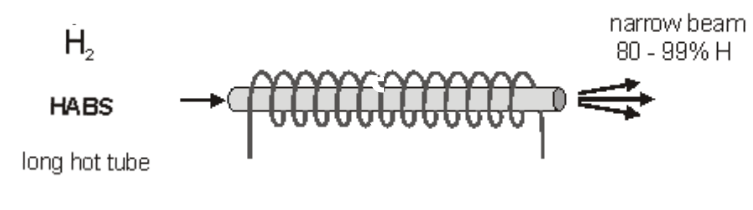
\includegraphics[width=0.5\textwidth]{doser}
  \caption{Graphical interpretation of the hydrogen atom beam source.\cite{HABS}}
  \label{HABS}
\end{figure}

\subsection{Sample Annealing and Graphene Repair}

The surface of the sample is kept clean by annealing to high temperatures by the filament in the manipulator. This ensures that contaminants on the surface are removed, in order to raise the quality of the STM images. After each dose of D$_2$ the sample was scanned by the STM. Hereafter the hydrogen, adsorbed on the surface, was removed by heating the sample above 900K. The graphene on the sample was checked, after cleaning the surface, in order to ensure that the number of defects was at a minimum. The size and shape of these are discussed in chapter \ref{cha:results}\\
If two many defects were present, the graphene on the sample was repaired by chemical vapour deposition (CVD), if a large number of defects were present on the surface. The sample was heated above 900\degree C in an ethylene pressure in the range of $1\cdot 10^{-6}$mbar. CVD growth of graphene is possible at temperatures above 1120 K, and the structural quality increases with the temperature.\cite{1367-2630-11-2-023006} During CVD the temperature of the sample surface was measured by an optical pyrometer, since the thermocouple measures the temperature on the backside of the Ir crystal. It is crucial that the Ir(111) surface is at least 1120K in order to break the ethylene bonds on the Ir(111) surface.\\
As a further study of the dissociation of hydrogen on graphene, bilayered graphene were grown on the Ir(111) surface. This was done according to the CVD procedure explained above. However, the sample was annealed for a long time (1-2 hours) during the growth of bilayers.

\section{TPD}

A quadrupole mass analyser is connected to the UHV chamber, and this was used to investigate the desorption of deuterium from the sample surface. The sample was positioned in the manipulator and heated by the filament as the experiments were carried out. From here the nozzle of the mass spec was brought within millimeters of the sample. The temperature was logged together with the amount of deuterium detected by the quadrupole. The mass spec was set to count masses of 4 amu, in order to exclude other molecules than deuterium. This setup was made with the computer program 'MASsoft' by Hiden Analytical.\\
A Eurotherm 2704 controller was used to control the current running through the filament in the manipulator. The controller was programmed to ramp the sample temperature from 300K to 900K at a rate of 1K per second. At maximum temperature the eurotherm was set to rest for 30s, and then slowly decrease current as the temperature dropped to a final temperature of 300K. This cycle was performed each time a TPD measurement was carried out. After this procedure all of the deuterium on the surface is desorbed from the sample.\\
As mentioned the temperature measured by the thermocouple is only valid for the backside of the sample. Therefore a calibration of the system is needed in order to find the correct peak temperatures. A calibration was done where the sample surface was measured with an optical pyrometer along with the thermocouple temperatures. Both temperatures were logged each time the temperature rose 30\degree C. The results from this calibration are seen in Figure \ref{TPDcalibration}. It is seen that there is no linear temperature ramp until the thermocouple reading is around 600K. This is due to the limitations of the pyrometer. The pyrometer measures the emitted radiation from a solid object, and in order to get a reading, the intensity of the emitted light from the measured object must be significant.\cite{pyrometer} However, a fit was made from the data points with a linear tendency. The fitted line had the following parameters:
\begin{align*}
  T_{surface} = T_{TC} * 0.7921 + 131.2
\end{align*}

\begin{figure}
  \centering
  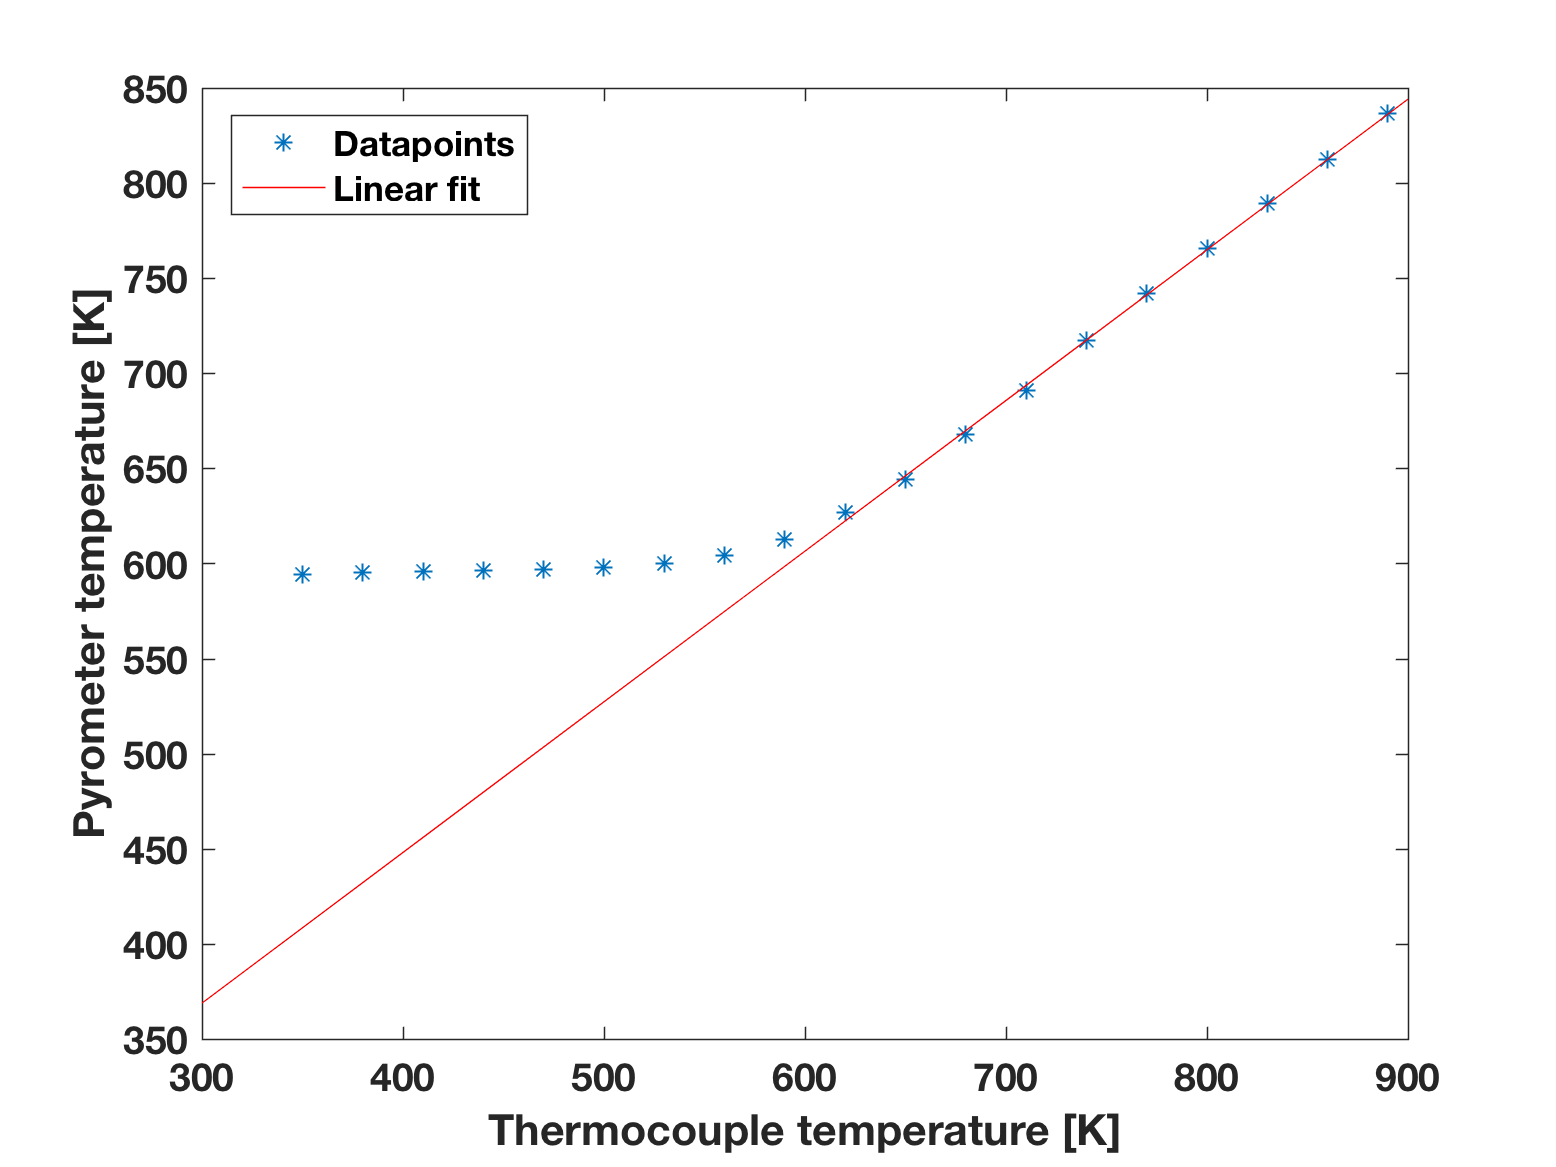
\includegraphics[width=0.55\textwidth]{TPD/kalibrering}
  \caption{Calibration of the temperature during the TPD measurements. The temperature of the surface measured by an optical pyrometer is plotted against the thermocouple temperature.}
  \label{TPDcalibration}
\end{figure}
In figure \ref{TPD:example} the data obtained from a typical TPD measurement is shown. Since the desorption of D$_2$ from the surface is investigated, a mass of 4 amu is monitored along with the temperature of the sample. It is seen that the temperature follows a linear ram. Some fluctuations are however seen in the beginning and end of the temperature interval. These measurements were carried out on the main graphene on Ir(111) sample.\\
During the last period of the project a new sample of graphene on Ir(111) was used to conduct TPD measurements. This sample had a freshly made monolayer of graphene.  This sample also had a thermocouple which seemed to have a loose connection, which caused problems with the temperature ramp. The readings from this thermocouple dropped out at some points, and generally seemed unstable. Furthermore, since the thermocouple was changed and a new sample holder was used, the Eurotherm controller parameters needed to be autotuned, in order to achieve a linear temperature ramp once again. This autotuning was unsuccessful, and the results from one of the TPD measurements from this sample can be seen in figure \ref{TPD:fail}. It is seen on figure \ref{TPD:example2} that the temperature ramp far from linear. The jumps in temperature do not seem to be systematic, which might indicate that the thermocouple as well as the controller parameters both had influence on the bad temperature ramp. The influence of the non linear ramp is also seen on the D$_2$ counts, where small peaks appear when the temperature changes rapidly. As seen on figure \ref{TPD:peak2} another peak appears right after the initial peak due to the jump in temperature. The initial peak was judged to fit the desorption of hydrogen best, and hence this peak value was used, as seen from the green circle in the figure. \\
Peak values were found by fitting a triple gaussian function to the data points around the peak. The initial peak value was estimated by visual observation, and the data points within $\pm$60\degree C are included in the fit. The temperatures at the maxima of the fits were determined, and these values are presented in chapter \ref{cha:results} as the peak temperatures. An example of the fit to the data points is shown in figure \ref{TPD:peak}. From this figure it is seen that the temperature at which the maximum counts number of counts are observed, not necessarily corresponds to the correct peak temperature. The green circle in figure \ref{TPD:peak} shows the found peak from which the sample temperature was gathered. These temperatures are found for each TPD measurement, and the desorption energy is estimated by the Redhead method described in chapter \ref{theory}.\\
In order to compare the individual peaks, the background was subtracted from every datapoint. The sample was positioned stationary in front of the nozzle and data was acquired for a period of time before each temperature ramp was started. These data points prior to the temperature ramp were used to calculate a mean background count, which was subtracted.

\begin{figure}[H]
  \centering
  \begin{subfigure}[b]{0.45\textwidth}
    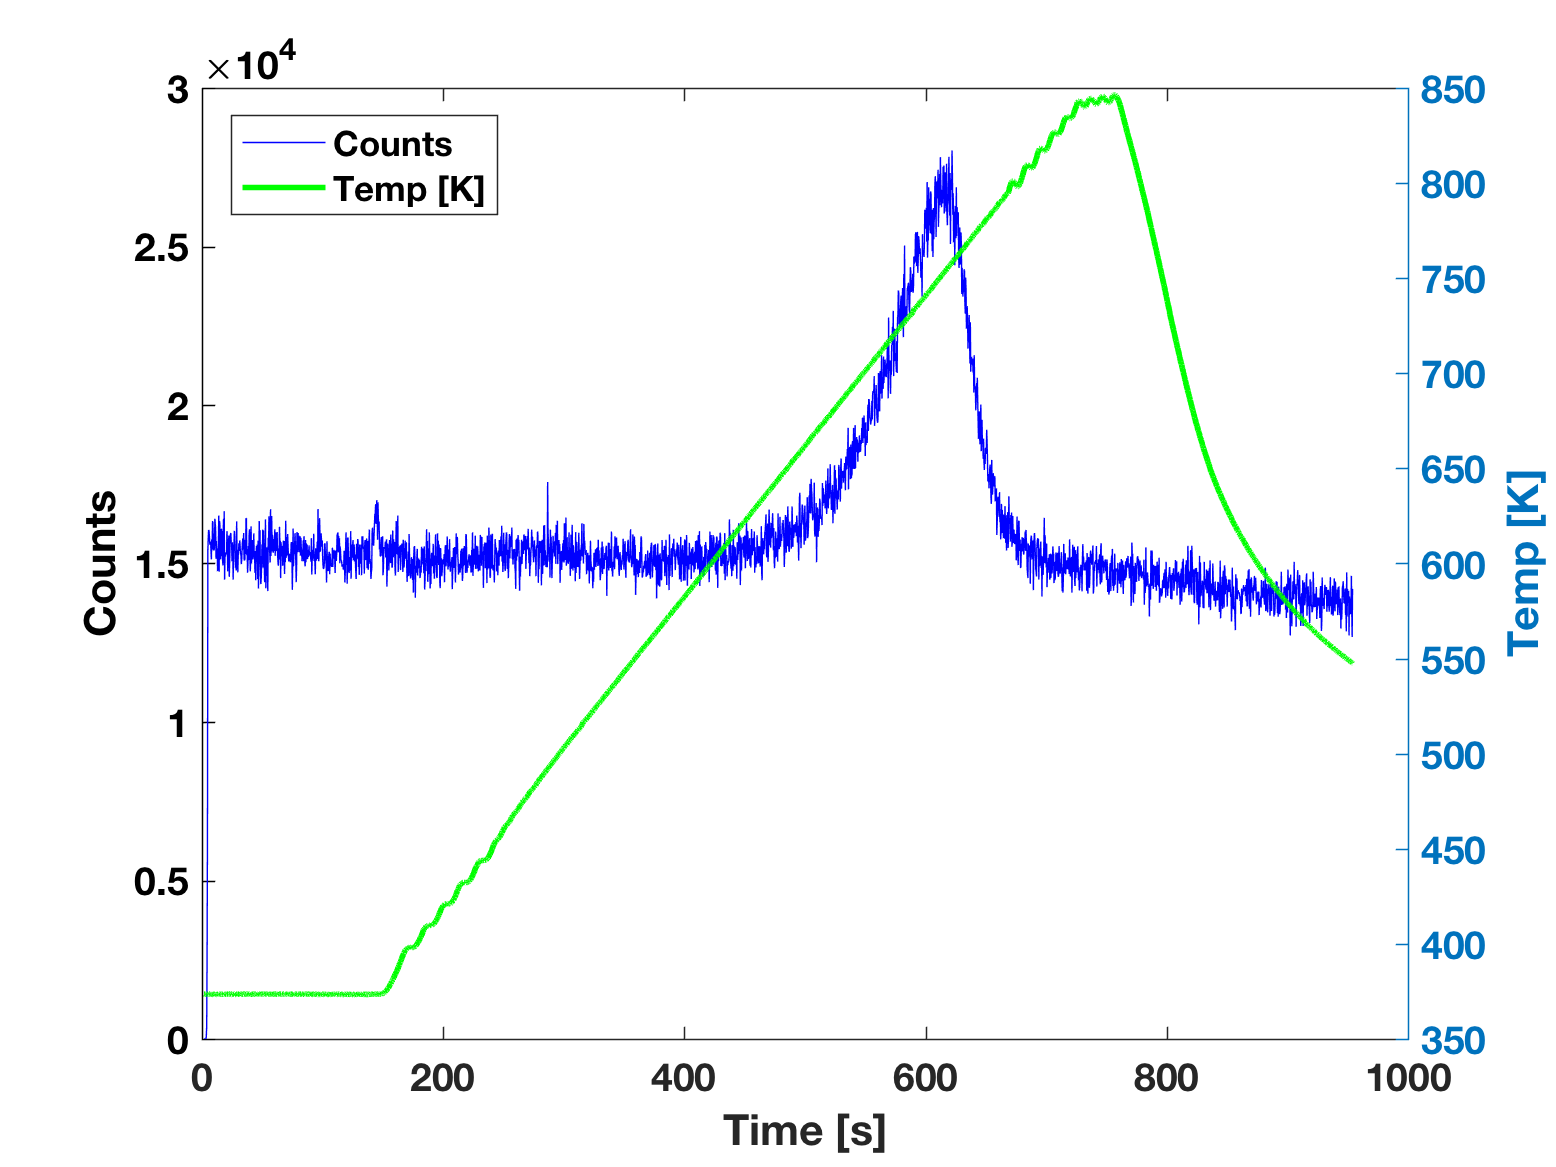
\includegraphics[width=\textwidth]{TPD/GrIr1740CD2_2504}
    \caption{}
    \label{TPD:example}
  \end{subfigure}
  \begin{subfigure}[b]{0.45\textwidth}
    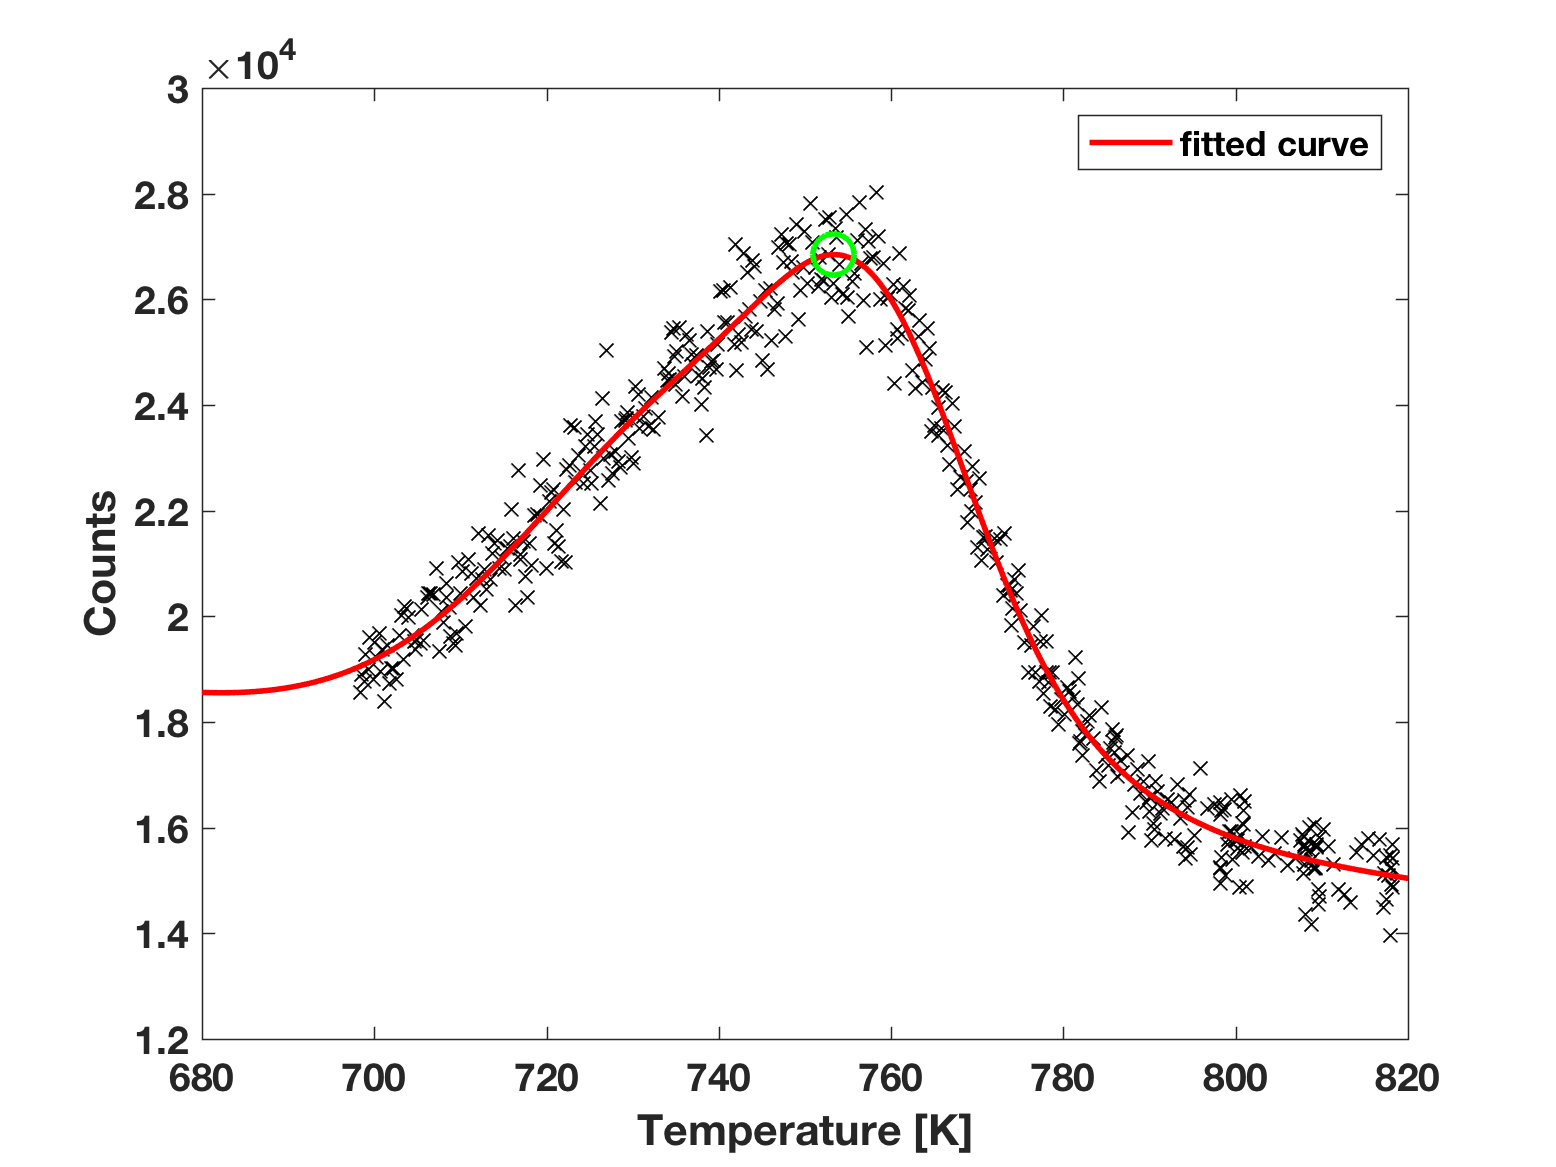
\includegraphics[width=\textwidth]{TPD/GrIr1740CD2_2504peak}
    \caption{}
    \label{TPD:peak}
  \end{subfigure}
  \caption{example of TPD measurements from the main sample. (a) shows data acquired from the quadrupole mass analyser and thermocouple readings. (b) shows the fitted curve to the datapoints within $\pm$60\degree C of the estimated peak value.}
  \label{TPD:win}
\end{figure}


\begin{figure}[H]
  \centering
  \begin{subfigure}[b]{0.45\textwidth}
    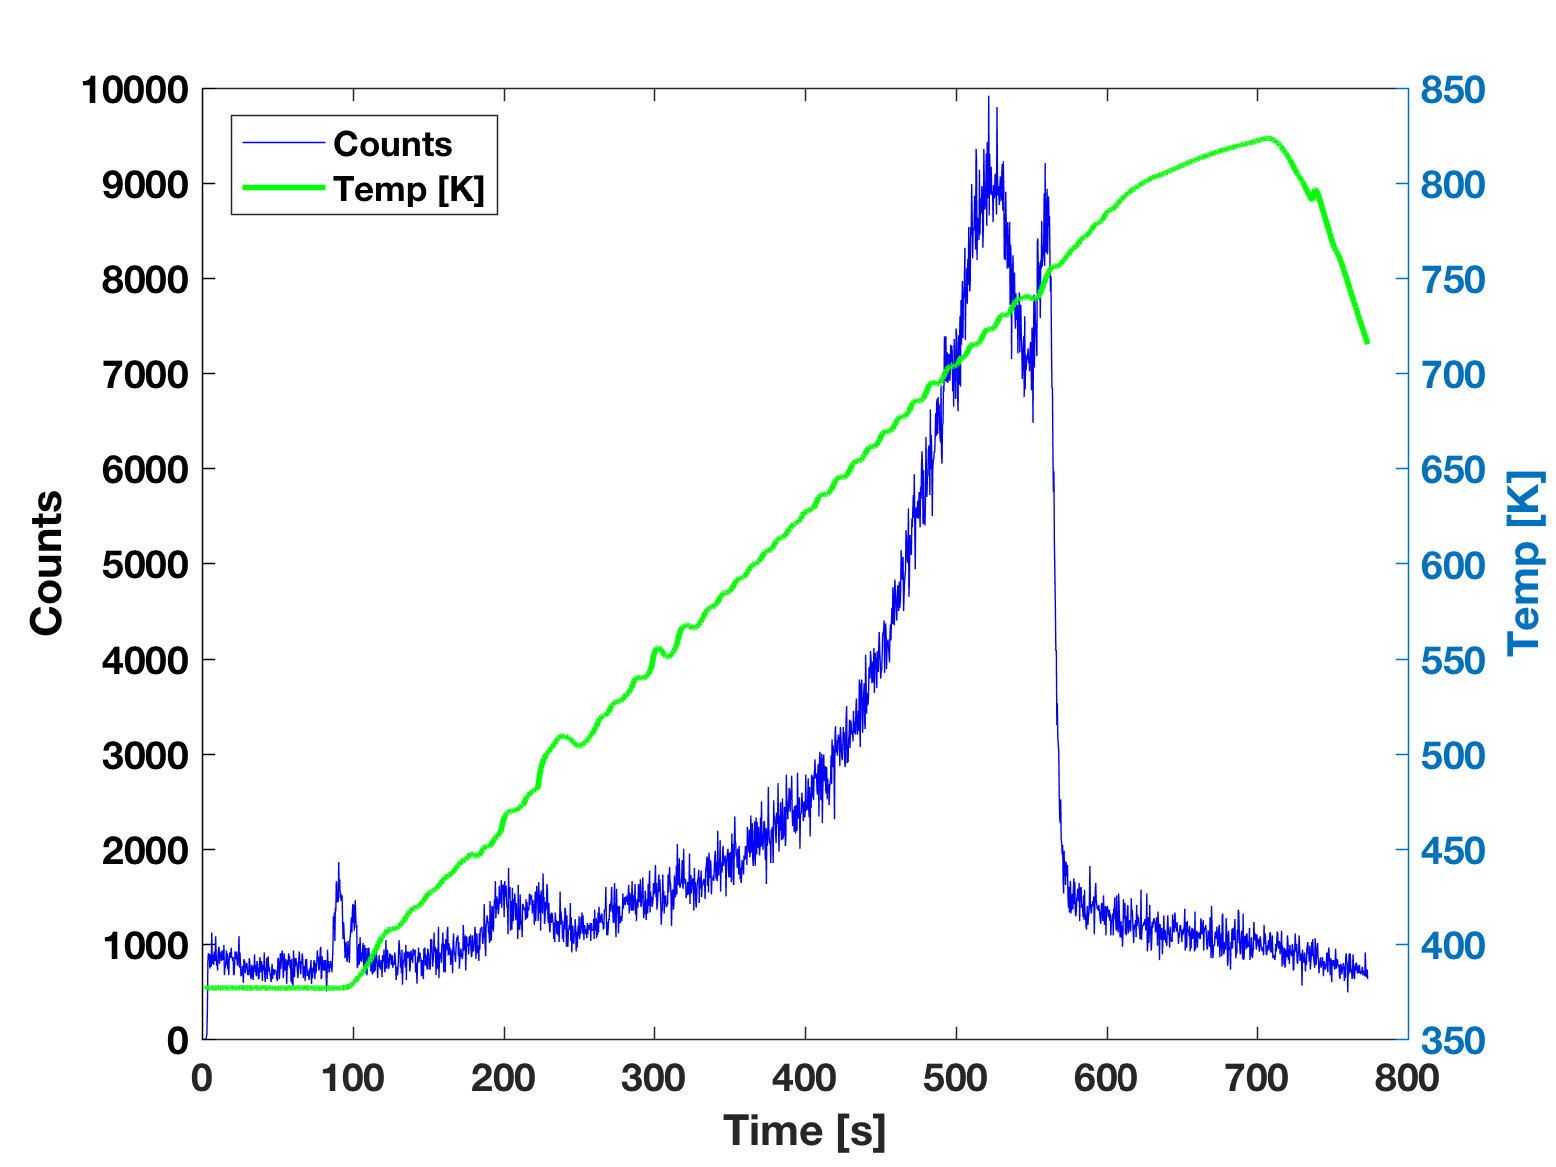
\includegraphics[width=\textwidth]{TPD/050516IrSorenD2dose1hour2}
    \caption{}
    \label{TPD:example2}
  \end{subfigure}
  \begin{subfigure}[b]{0.45\textwidth}
    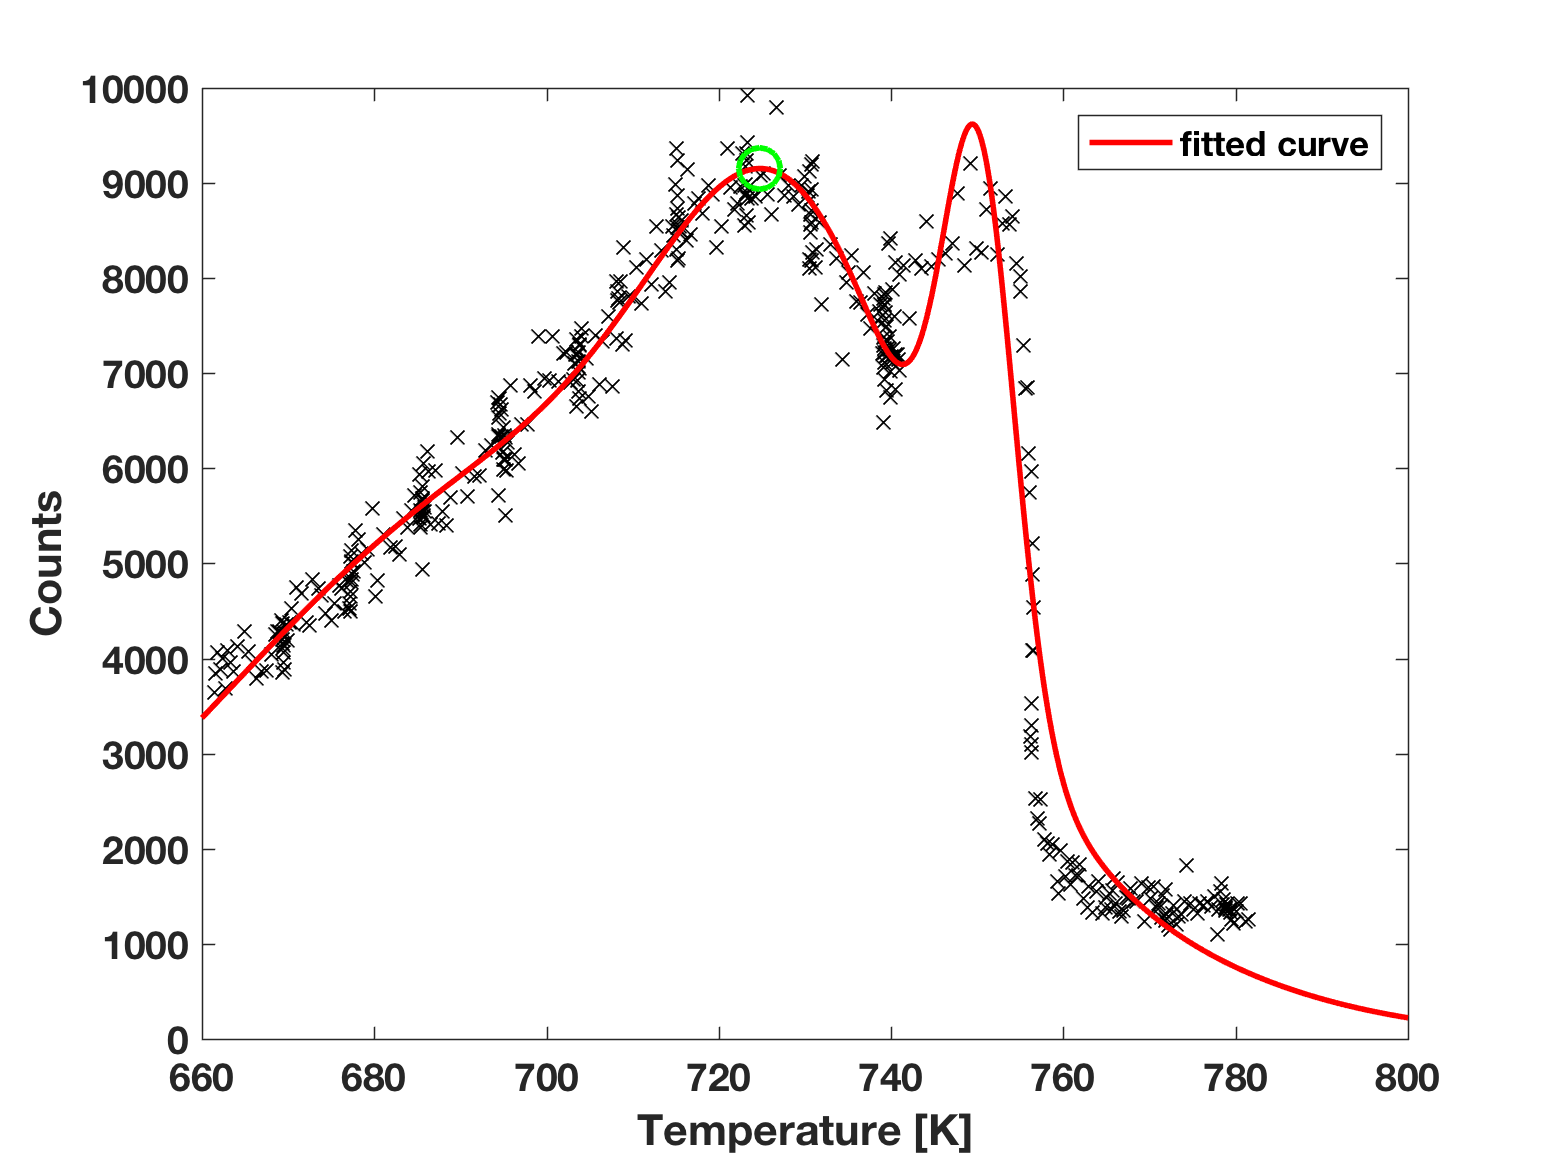
\includegraphics[width=\textwidth]{TPD/050516IrSorenD2dose1hour2peak}
    \caption{}
    \label{TPD:peak2}
  \end{subfigure}
  \caption{example of TPD measurements from the new sample. (a) shows data acquired from the quadrupole mass analyser and thermocouple readings. (b) shows the fitted curve to the datapoints within $\pm$60\degree C of the estimated peak value.}
  \label{TPD:fail}
\end{figure}
